\documentclass[11pt]{article}
%\documentclass[12pt]{amsart}
%\usepackage{latex8}
\usepackage{fullpage}
\usepackage{times}
\usepackage{url}
\usepackage[normalem]{ulem}
\usepackage{epsfig} 
%\usepackage{latexsym}
\usepackage{subfigure}
\usepackage{graphicx}
\usepackage{titlesec}
\usepackage{multirow}

\titlespacing{\section}{0pt}{3mm}{1mm}
\titlespacing{\subsection}{0pt}{2mm}{0.5mm}
\titlespacing{\subsubsection}{0pt}{2mm}{0.8mm}

%\topmargin 0.75in 
%\oddsidemargin -0.04in
%\textwidth 6.5in
%\textheight 9.0in 
%\setlength{\textheight}{23.1cm}
%\setlength{\textwidth}{17.0cm}

\newcommand{\muhat}{\hat{\mu}}
\newcommand{\sigmahat}{\hat{\sigma}}
\newcommand{\todo}[1]{[\textbf{TODO: #1}]}
\newcommand{\eat}[1]{} % TO MAKE LARGE BLOCKS OF TEXT INVISIBLE
\newcommand{\sz}[1]{\lvert#1\rvert}
\newcommand{\card}[1]{\lvert#1\rvert}
\newcommand{\xp}[2]{P \if*#1\else^{#1}\fi \if*#2\else_{\! #2}\fi}
\newcommand{\pr}[3]{\xp{#1}{#2}\left\{\,#3\,\right\}}
\newcommand{\prl}[3]{\xp{#1}{#2}\{\,#3\,\}}
\renewcommand\:{\colon} % for use with \sset, etc.
\newcommand{\sset}[1]{\left\{\,#1\,\right\}}
\newcommand\xD{\mathcal{D}}
\newcommand\xP{\mathcal{P}}
\newcommand\xS{\mathcal{S}}
\newcommand\xbar{\bar x}
\newcommand\vbar{\bar v}
\newcommand\xmax{{x_{\text{max}}}}
\newcommand\eps{\epsilon}
\newcommand{\eeblk}{\hbox{\lower 1pt \vbox{\hrule width6pt\hbox to
  6pt{\vrule height5pt depth1pt \hfil\vrule height5pt depth1pt} \hrule
  width6pt} \unskip}}
\newcommand{\eblk}{{\unskip\nobreak\hfil\penalty50
  \hskip1em\hbox{}\nobreak\hfil\eeblk
  \parfillskip=0pt\finalhyphendemerits=0\par}}
\newtheorem{xample}{Example}
%\newenvironment{example}{\begin{xample}\em}{\eblk\end{xample}}
\makeatletter
\newenvironment{sql}%
 {\vskip 5pt\begin{list}{}{%
  \setlength{\topsep}{0pt}\setlength{\partopsep}{0pt}\setlength{\parskip}{0pt}%
  \setlength{\parsep}{0pt}\setlength{\labelwidth}{0pt}%
  \setlength{\rightmargin}{0pt}\setlength{\leftmargin}{0pt}%
  \setlength{\labelsep}{0pt}%
  \obeylines\@vobeyspaces\normalfont\ttfamily%
  \item[]}}
 {\end{list}\vskip5pt\noindent}
\makeatother
\newcommand{\bpar}[1]{\vskip 5pt\noindent\textbf{#1}\hskip 1em}
\newcommand\yN{{\tilde N}}
\newcommand\yX{{\tilde X}}
\newcommand\ymu{{\tilde\mu}}
\newcommand\ysigma{{\tilde\sigma}}


\newcommand{\goodgap}{
        \hspace{\subfigtopskip}
        \hspace{\subfigbottomskip}
}

%\renewcommand{\baselinestretch}{0.99}

\newtheorem{definition}{Definition}
\newtheorem{Rule}{Rule}
\newtheorem{lemma}{Lemma}
\newtheorem{theorem}{Theorem}
\newtheorem{problem}{Problem}
\newtheorem{example}{Example}
\newtheorem{optimization}{Optimization}
\newtheorem{observation}{Observation}
\newtheorem{corollary}{Corollary}

\newcommand{\qed}{\hspace*{\fill}
           \vbox{\hrule\hbox{\vrule\squarebox{.667em}\vrule}\hrule}\smallskip}

\long\def \ignoreme#1{}

\def\qed{\hfill \mbox{\rule[0pt]{1.5ex}{1.5ex}}}



\begin{document}
%\maketitle
%\pagestyle{empty}

\begin{center}
{\bf \huge{COMP 543 Assignment \#6: Deep Learning with TensorFlow}}
\end{center}

%\noindent Due Wednesday, May 2nd at 5:00 PM. Note that this is the absolute latest possible date \& time we can have the assignment due, so no normal extensions will be granted.

\section*{Description}
The learning objectives of this assignment are to give you experience specifying neural network architectures, training the neural networks,  and seeing how well they perform on an image recognition task.

In this assignment, you will be using Google's open-source TensorFlow machine learning tool via Keras to implement
some deep learning architectures that will be used to classify images as one of four different cell types. 

Read the entire assignment before starting! 

%Since deep learning is computationally expensive, it is strongly recommended that you use one of Amazon's deep learning machines to do this assignment (see below). 
%, but might take XX times as long (or more) using a laptop. 
%Plus, Keras/TensorFlow can be a bit of a pain to install on your laptop, so using Amazon is just plain easier. The only situation in which you might consider using your own hardware is if you've got a tricked out laptop/desktop with a beefy GPU for game playing that TensorFlow can make use of.


\section*{Honor Code}

You make work fully collaboratively with your team members. You may discuss the assignment at a high level with other people in the course. However, you may not share code in any way (viewing, verbally, etc.) with non-team members.  You may use the Internet to look up syntax for Keras commands but may not use it to search for answers to the problems. If you are unsure of what is allowed, ask!

\subsection*{Working with a Partner}
For this assignment, unlike previous assignments, you are welcome to work with a partner. You don't
have to work with a partner; the assignment is doable without one. We estimate 10-15 hours of work for an
average student to complete all of the tasks.
If you do work with a partner, make sure to put \textbf{both} partner's names in the write-up you submit.
And only \textbf{one} partner should turn in the assignment.


\section*{AWS  (review of TensorFlow Lab)}
This assignment must be completed on AWS. Please do not use comp543.clear.rice.edu as the machine does not have sufficient power.

\subsection*{Running TensorFlow on AWS }

Follow these steps:
\begin{enumerate}
\item  Log on to Amazon AWS Educate and go to your AWS console
\item Click on ``EC2''
\item Click on ``Launch Instance''. You will be asked for a machine instance to start up (this will govern the software on the machine you run).
\item Scroll down to ``Deep Learning AMI (Ubuntu)'' and click ``Select''. This machine instance (not
surprisingly, given the name) has a number of deep learning tools installed on it. 
\item Choose the machine type you will rent. Choose ``t2.xlarge''  
\item Click ``Review and Launch''
\item Click ``Launch''
\item Select the appropriate key file and acknowledge access
%You will want to choose a machine with a GPU, which will make your deep learning codes much faster. Choose ``p2.xlarge'' 
% You want to make sure that you can SSH into your machine, so choose ``Edit Security Groups'' then click ``Add Rule'' to make sure to allow SSH access from Anywhere. Once you have done that, click ``Review and Launch'' and then ``Launch''. 
\item You can find your running instance by going to the EC2 Dashboard and then clicking on ``Running Instances''.

\item Copy the images to the machine using \texttt{scp}. The \texttt{-r} flag will copy recursively

%{\small
%\texttt{scp -i "myPemFile.pem" /path/file/*.jpeg ubuntu@myDNS.compute-1.amazonaws.com:}\\
%}

\item SSH into your machine (just like for EMR), You can find the connection string to connect to your machine by clicking on the ``Connect" button

\item Start tensorflow:

\texttt{source activate tensorflow\_p36}\\

\item Run your code interactively or in batch using python

\item As usual, when you are done with your machine, \textbf{MAKE SURE TO SHUT IT DOWN!!}
\end{enumerate}

The learning problems we'll consider will take about 30 minutes each using one of these machines


%
%\subsection{Running TensorFlow on Google Colab }
%
%You may complete this assignment using Google Colab. Please note that we cannot guarantee availability of Colab, so please allow enough time to complete the assignment on AWS, if, for some reason, Colab is not available.
%
%If you use Google Colab, you will need to create a new Colab notebook that contains your code and results. You may modify the Colab notebook from the TensorFlow lab, if you like.

\subsection*{What to Turn in}
%Submit  your new Colab notebook (.ipynb file with all of the tasks and outputs).  You may submit your answers to questions and the tables in a PDF.

Submit a zip file containing:
\begin{enumerate}
\item A python file (.py) with your code
\item A filled-out Excel spreadsheet with your write-up.  DO NOT ADD OR REMOVE LINES FROM THE SPREADSHEET!  If you need to make additional comments, please do so in a separate file. We are automatically processing the csv version of this file and any changes you make are likely to break our process.
\item A standard csv version of your spreadsheet. In my version of Excel, you can get this with Save As>Comma Separated Values. NOT CSV UTF-8.
\item A text capture of the output of your running code output. You may submit a separate file for each model, if you like.
\end{enumerate}

\section*{The Data}
There are 12,515 images, each 320 x 240 pixels in size. Each image contains one cell type, either  eosinophil, lymphocyte, monocyte, or neutrophil.  The image labels are contained in bloodcellLabels.csv.

The dataset may be found here:

\url{https://www.kaggle.com/paultimothymooney/blood-cells}


Download the data. Use the dataset2-master files. Train your model on the images in the folder named \texttt{TRAIN} and test your model on the images in the folder named \texttt{TEST}. We will not be using the images in the folder named \texttt{TEST\_SIMPLE}.

Each image contains an RGB (red-green-blue) channel value for each pixel. 

\section*{Our Results}
For comparison, the results we obtained on this assignment were:


    \begin{center}
     \begin{tabular}{l|cccc}
         \hline
         Type & time per epoch (sec) & loss & training accuracy & 
testing accuracy \\
         \hline
         Dense FFNN        & 13.23 & 1.3863             & 0.2494 & 0.2505 \\
         CNN               & 15.46 & 0.0013             & 1.0000 & 0.4962 \\
         Modified CNN      & 19.37 & $2 \times 10^{-5}$ & 1.0000 & 0.4757 \\
         Our lazy best CNN & 17.77 & 0.0351             & 0.9879 & 0.7692 \\
         \hline
     \end{tabular}
     \end{center}
     
 

\section*{The Code}
We have provided you with code that reads the images in by RGB channel as well as skeleton code to run your models.

 You will need to construct deep learning networks that generate  sets of probabilities for each image, indicating how likely each image is to contain each of the four cell types. 
 
 \section*{Output}
 
 Once you have your code running, you can run it directly from the command line and redirect the output to both a file and the screen using the following command (Note: there is no space between $>$ and \&:
 
 \texttt{python myprogramname.py $>\&1\ |$ tee myoutputfilename.txt}

\section*{The Tasks}
There are 4 separate tasks that you need to complete to finish the assignment.

\section{Task 1: Feed forward network}
\subsection{A: (20 points) Construct a feed forward network}

Construct a single hidden layer feed forward network with the following parameters / characteristics:

\begin{itemize}
\item Downsample the images via average pooling by a factor of 4, using `same' padding
\item 16 nodes in the hidden layer
\item relu activation function
\item 100 training epochs
\item Batch size of 64
\item Adam optimizer
\item Compute accuracy as an additional metric
\item Categorical\_crossentropy loss function
\item Softmax output layer
\end{itemize}

Train your model.

Be sure to time the training step, as you will need to report this information.

This figure depicts the components of a basic feed forward network.

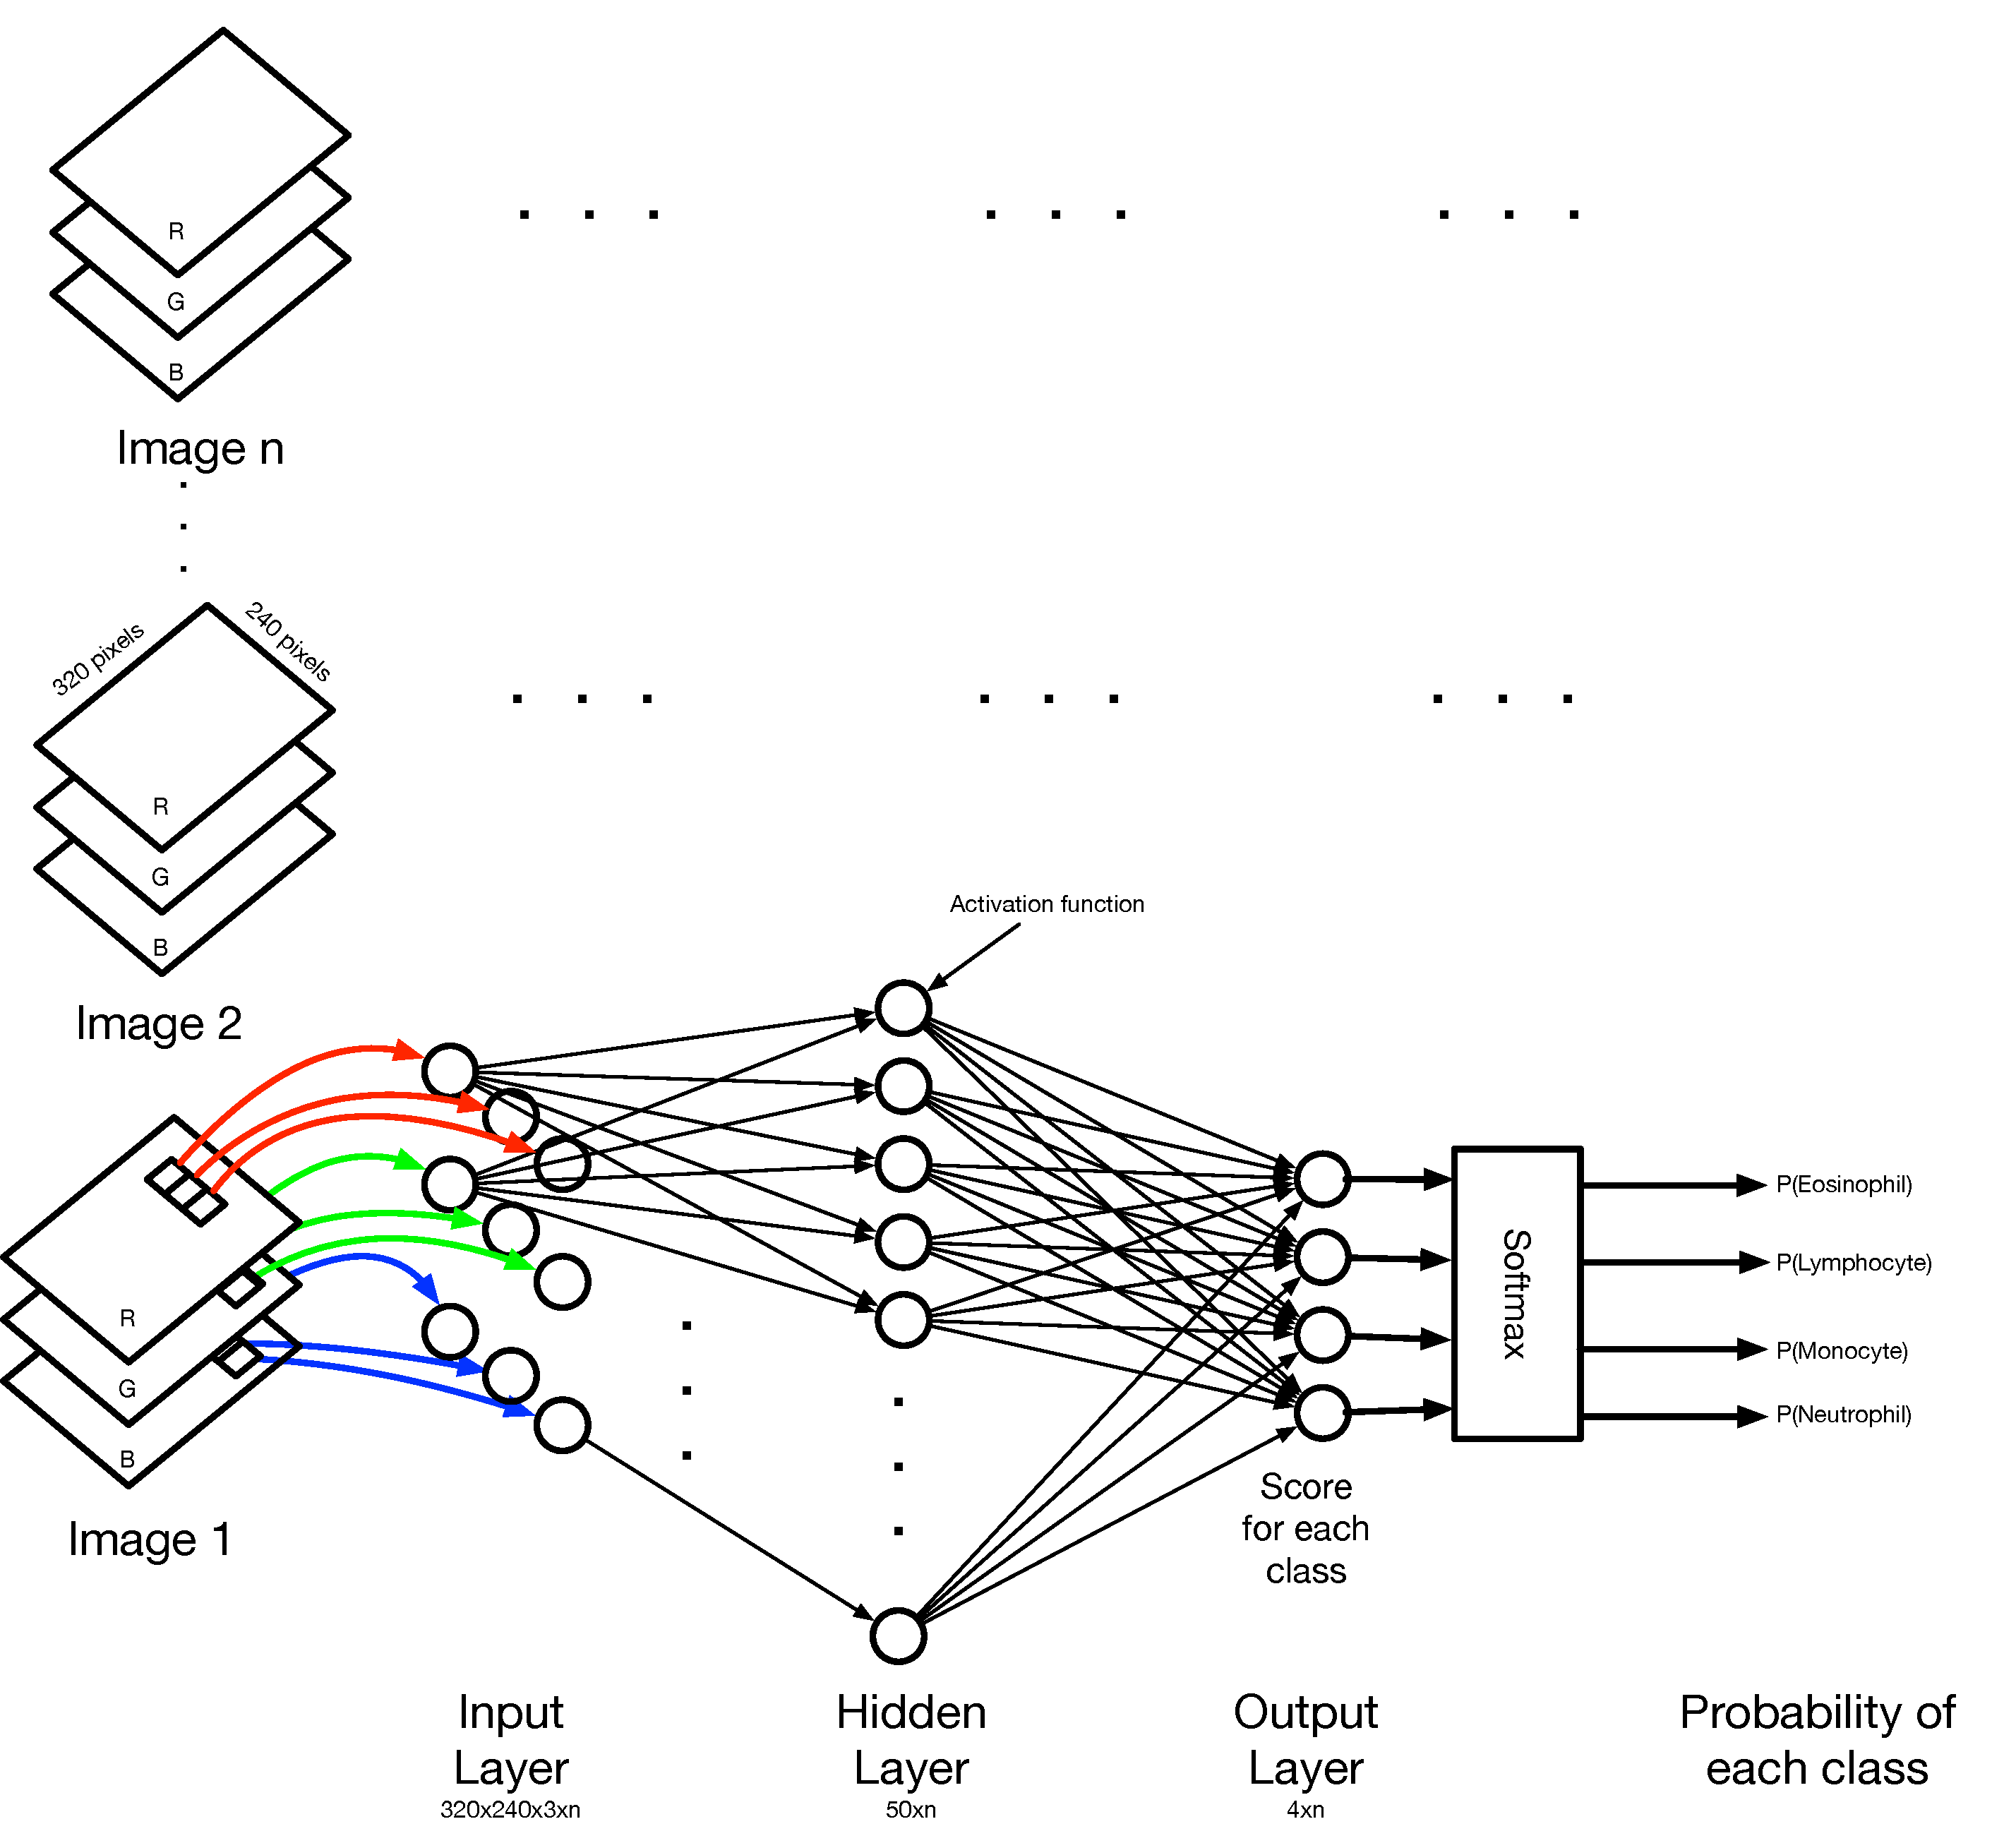
\includegraphics[width=0.6\textwidth]{FF.pdf}

Note that you need a mapping from the image pixels to the input layer. Many such mappings are possible. One is:

\includegraphics[width=0.4\textwidth]{ffmap.pdf}

which can be obtained with the \texttt{Flatten} function in Keras.



\subsection{B: (10 points) Compute results for your feed forward network}

Please record your answers in the provided spreadsheet. Questions are repeated here for your reference. You may compute metrics (e.g. sensitivity, specificity, etc.) using equations in the spreadsheet, or you may write code to compute the metrics.

Please do NOT modify the results spreadsheet (other than possibly adding formulas) and please use a single cell for each answer.  This format should help us combine results for reporting.

\noindent For this network:
\begin{enumerate}
\item What was the accuracy on the training data at the final epoch? 

\item Time the training step. How many minutes did it take to train your model?

\item Populate the following confusion matrix, showing the counts for each class

\begin{tabular}{|l|c|c|c|c|c|c|} \hline
\multicolumn{2}{|c|}{ } &  \multicolumn{5}{|c|}{\textbf{Predicted}}  \\ \cline{3-7}
\multicolumn{2}{|c|}{ } & \textbf{Eosinophil} & \textbf{Lymphocyte} & \textbf{Monocyte} & \textbf{Neutrophil} & \textbf{Total}   \\ \hline
\multirow{ 4}{*}{\textbf{Actual}}& \textbf{Eosinophil}  & & & & & \\ \cline{2-7}
& \textbf{Lymphocyte}    & & & & & \\ \cline{2-7}
& \textbf{Monocyte}    & & & & & \\ \cline{2-7}
& \textbf{Neutrophil}   & & & & &\\ \cline{2-7}
& \textbf{Total} & & & & & \\ \hline
\end{tabular}

\item Fill in the following table of metrics


\begin{tabular}{|l|c|c|c|c|c|c|} \hline
\textbf{Cell Type} & \textbf{\% Correct} & \textbf{Sensitivity (Recall)} & \textbf{Specificity} & \textbf{Precision} & \textbf{F1} & \textbf{F2} \\ \hline
Eosinophil & & & & & & \\ \hline
Lymphocyte &  & & & & & \\ \hline
Monocyte &  & & & & & \\ \hline
Neutrophil & & & & & & \\ \hline
\end{tabular}
\item Which cell type was most predictable? Justify your answer.
%\vspace{2 em}


\item If you worked with a partner, describe the breakdown of work:

%\vspace{3cm}
\end{enumerate}


\section{Task 2: Convolutional Neural Network}
\subsection{A: (10 points) Create the CNN}

Starting with the feed forward network you created, replace the dense layer with a convolution layer with a 3 x 3 kernel and \texttt{same} padding.

Train your model.

\subsection{B: (10 points) Compute results for your CNN}

Please record your answers in the provided spreadsheet. Questions are repeated here for your reference. You may compute metrics (e.g. sensitivity, specificity, etc.) using equations in the spreadsheet, or you may write code to compute the metrics.

\begin{enumerate}
\item What was the accuracy on the training data at the final epoch? 

\item Time the training step. How many minutes did it take to train your model?

\item Populate the following confusion matrix, showing the counts for each class

\begin{tabular}{|l|c|c|c|c|c|c|} \hline
\multicolumn{2}{|c|}{ } &  \multicolumn{5}{|c|}{\textbf{Predicted}}  \\ \cline{3-7}
\multicolumn{2}{|c|}{ } & \textbf{Eosinophil} & \textbf{Lymphocyte} & \textbf{Monocyte} & \textbf{Neutrophil} & \textbf{Total}   \\ \hline
\multirow{ 4}{*}{\textbf{Actual}}& \textbf{Eosinophil}  & & & & & \\ \cline{2-7}
& \textbf{Lymphocyte}    & & & & & \\ \cline{2-7}
& \textbf{Monocyte}    & & & & & \\ \cline{2-7}
& \textbf{Neutrophil}   & & & & &\\ \cline{2-7}
& \textbf{Total} & & & & & \\ \hline
\end{tabular}

\item Fill in the following table of metrics


\begin{tabular}{|l|c|c|c|c|c|c|} \hline
\textbf{Cell Type} & \textbf{\% Correct} & \textbf{Sensitivity (Recall)} & \textbf{Specificity} & \textbf{Precision} & \textbf{F1} & \textbf{F2} \\ \hline
Eosinophil & & & & & & \\ \hline
Lymphocyte &  & & & & & \\ \hline
Monocyte &  & & & & & \\ \hline
Neutrophil & & & & & & \\ \hline
\end{tabular}
\item Which cell type was most predictable? Justify your answer.
%\vspace{2 em}


\item If you worked with a partner, describe the breakdown of work:

%\vspace{2 em}

\item Which network performed better, the feed forward or the convolutional? Justify your answer.


\end{enumerate}


\section{Task 3: Modify the CNN}
\subsection{A: (10 points) Modify the CNN}

There are a number of ways in which the existing network can be improved.  Make a \textbf{single} change to the network and recompute the confusion matrix and metrics.   Possible changes include:

\begin{itemize}
\item Change the size of the images being used (specify)
\item Change the size of the convolution kernel (specify)
\item Handle image edges differently (specify)
\item Change the number of hidden nodes (specify)
\item Change the activation function (specify) 
\item Change the optimizer (specify)
\item Add another convolutional layer (specify where, how many nodes, activation function used, kernel size, padding)
\item Add a pooling layer
\item Add a dropout layer (specify)
\item Add a batch normalization layer
\item Change the learning rate (specify)
\end{itemize}

Check the course discussion to ensure that your (team's) change is unique. Multiple teams may make similar changes (e.g. the number of hidden nodes) but each team making the same type of change must use a different parameter value.  The first team to claim a modification and parameter value will get credit for that change.

\subsection{B: (10 points) Compute results for your modified CNN}

\begin{enumerate}
\item Describe the single change you made.  
\item Why did you choose this change?  For example, if you change the optimizer, why do you think the new optimizer will be better?
\item What made you believe it would improve the model?  
\item In what way(s) did you expect it to impact the model?
\item What was the accuracy on the training data at the final epoch? 

\item Time the training step. How many minutes did it take to train your model?

\item Populate the following confusion matrix, showing the counts for each class

\begin{tabular}{|l|c|c|c|c|c|c|} \hline
\multicolumn{2}{|c|}{ } &  \multicolumn{5}{|c|}{\textbf{Predicted}}  \\ \cline{3-7}
\multicolumn{2}{|c|}{ } & \textbf{Eosinophil} & \textbf{Lymphocyte} & \textbf{Monocyte} & \textbf{Neutrophil} & \textbf{Total}   \\ \hline
\multirow{ 4}{*}{\textbf{Actual}}& \textbf{Eosinophil}  & & & & & \\ \cline{2-7}
& \textbf{Lymphocyte}    & & & & & \\ \cline{2-7}
& \textbf{Monocyte}    & & & & & \\ \cline{2-7}
& \textbf{Neutrophil}   & & & & &\\ \cline{2-7}
& \textbf{Total} & & & & & \\ \hline
\end{tabular}

\item Fill in the following table of metrics


\begin{tabular}{|l|c|c|c|c|c|c|} \hline
\textbf{Cell Type} & \textbf{\% Correct} & \textbf{Sensitivity (Recall)} & \textbf{Specificity} & \textbf{Precision} & \textbf{F1} & \textbf{F2} \\ \hline
Eosinophil & & & & & & \\ \hline
Lymphocyte &  & & & & & \\ \hline
Monocyte &  & & & & & \\ \hline
Neutrophil & & & & & & \\ \hline
\end{tabular}
\item Which cell type was most predictable? Justify your answer.
%\vspace{2 em}


\item If you worked with a partner, describe the breakdown of work:

%\vspace{2 em}

\item Did this model perform better than the basic CNN? Justify your answer.

\end{enumerate}

\section{Task 4: Improve your CNN}

Make \textbf{at least} one more change to your modified CNN to try and improve the model.  If you feel that the results for your modified CNN decreased performance, you may start over with the basic CNN and make at least two changes.

The goal here is to see how good you can get your model to perform.

You can make a number of single changes, progressively (hopefully) improving the model, or you may make multiple changes at once. When you make multiple changes at the same time it can be difficult to tell which change caused the new results.

\subsection{A: (10 points) Improve the CNN}

There are a number of ways in which the existing network can be improved.  Make  \textbf{changes} to the network and recompute the confusion matrix and metrics.   


\subsection{B: (10 points) Compute results for your improved CNN}

Give us your best results below. You do not need to report results for intermediary models (though you may find it beneficial to record them. If you record intermediary results, please do so on a second spreadsheet and submit it with your assignment. It will be interesting to see what you did.


\begin{enumerate}
\item Describe the change(s) you made.
\item Why did you choose these changes?  For example, if you change the optimizer, why do you think the new optimizer will be better?
\item What made you believe they would improve the model?  
\item In what way(s) did you expect it to impact the model?
\item What was the accuracy on the training data at the final epoch? 

\item Time the training step. How many minutes did it take to train your model?

\item Populate the following confusion matrix, showing the counts for each class

\begin{tabular}{|l|c|c|c|c|c|c|} \hline
\multicolumn{2}{|c|}{ } &  \multicolumn{5}{|c|}{\textbf{Predicted}}  \\ \cline{3-7}
\multicolumn{2}{|c|}{ } & \textbf{Eosinophil} & \textbf{Lymphocyte} & \textbf{Monocyte} & \textbf{Neutrophil} & \textbf{Total}   \\ \hline
\multirow{ 4}{*}{\textbf{Actual}}& \textbf{Eosinophil}  & & & & & \\ \cline{2-7}
& \textbf{Lymphocyte}    & & & & & \\ \cline{2-7}
& \textbf{Monocyte}    & & & & & \\ \cline{2-7}
& \textbf{Neutrophil}   & & & & &\\ \cline{2-7}
& \textbf{Total} & & & & & \\ \hline
\end{tabular}

\item Fill in the following table of metrics


\begin{tabular}{|l|c|c|c|c|c|c|} \hline
\textbf{Cell Type} & \textbf{\% Correct} & \textbf{Sensitivity (Recall)} & \textbf{Specificity} & \textbf{Precision} & \textbf{F1} & \textbf{F2} \\ \hline
Eosinophil & & & & & & \\ \hline
Lymphocyte &  & & & & & \\ \hline
Monocyte &  & & & & & \\ \hline
Neutrophil & & & & & & \\ \hline
\end{tabular}
\item Which cell type was most predictable? Justify your answer.
%\vspace{2 em}


\item If you worked with a partner, describe the breakdown of work:

%\vspace{2 em}

\item Did this model perform better than your modified CNN? Justify your answer.

\end{enumerate}
%\section{Follow-up}
%
%\begin{enumerate}
%\item Which task was most helpful to your learning
%
%On a scale of 1 to 5, with 1 being not much  and 5 a lot
%\item  My understanding of Feed Forward Neural Networks has increased
%\item  My understanding of Convolutional Neural Networks has increased
%\item  My understanding of Confusion Matrices has increased
%\item  My understanding of accuracy measures has increased
%% how much of the assignment did they complete?
%% which part did each person complete?
%\item Working in pairs contributed to the learning of this material
%
%\end{enumerate}
%

\end{document}
